\documentclass[a4paper,12pt, spanish, twocolumn]{article}

% Para trabajar en idioma español
\usepackage[T1]{fontenc}
\usepackage{selinput}
\usepackage{babel}
\SelectInputMappings{%
  aacute={á},
  ntilde={ñ},
  Euro={€}
}
%%%%%%%%%%%%
\usepackage{blindtext} %libreria que nos permite generar texto "tonto"
\usepackage{graphicx} %libreria que nos permite ingresar las imagenes


\begin{document}
	\title{Ejemplo 6}
	\author{Nombre del autor}
	\date{Febrero 14, 2015}
	\maketitle
	\begin{abstract}
	\blindtext
	\end{abstract}
	\section{Primera sección}
	\blindtext
	
	\begin{quote}
		\blindtext
	\end{quote}
	\blindtext
	
	\begin{table}[h]
		\centering
		\begin{tabular}{| c || l |}
	    	\hline \hline
	     	No. & Nombre \\
     		\hline \hline
      		1 & Lunes \\
      		2 & Martes \\
	      	3 & Miércoles \\
    	  	4 & Jueves \\
      		5 & Viernes \\
	      	6 & Sábado \\
    	  	7 & Domingo \\
      		\hline
		  \end{tabular}
  		\caption{Días de la semana}
	\end{table}


	\section{Segunda sección}
		\blindtext[1]
		%	El comando \ref{nombre_imagen} nos permite referenciar graficos, secciones, etc.

		Como se puede ver en la Fígura \ref{fig:bellcurve}.
		\begin{figure}[ht]
		    \centering %centra la imagen segun el ancho de la columa
		    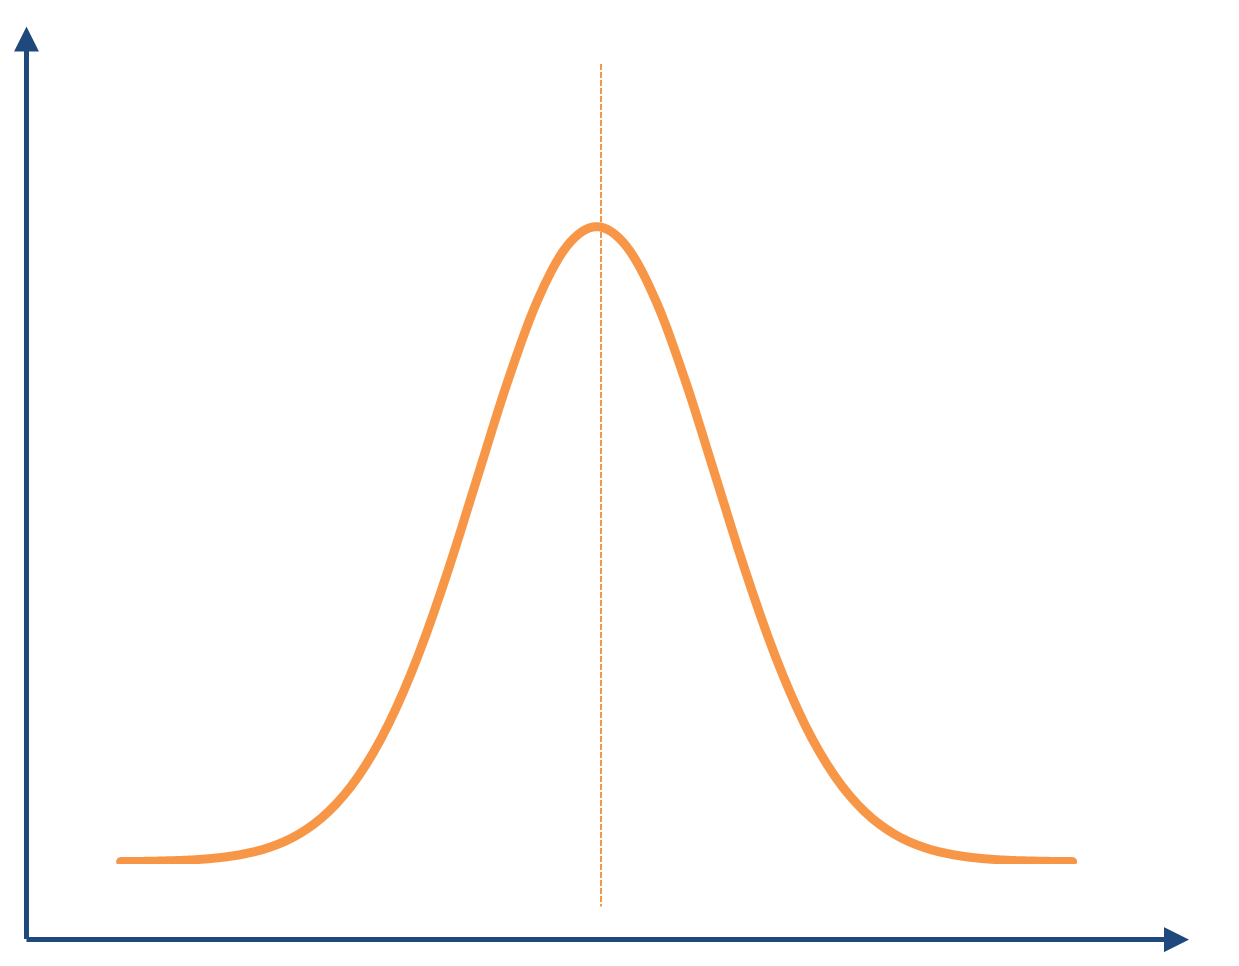
\includegraphics[scale=0.3]{BellCurve.png}
		    \caption{Figura que muestra una curva en forma de campana}
    		\label{fig:bellcurve} %asigna un nombre a la imagen (en caso de que se necesite referenciarlo dentro del documento)
		\end{figure}

		\subsection{Esta es una subsección}
			\blindtext[5]
			Como se puede ver en la ecuación \ref{eq:1}.
			\\\\
			\noindent
			$ \lim_{x \to \infty} \exp(-x) = 0 $
			
			\begin{equation} \label{eq:1}
			\lim_{x \to \infty} \exp(-x) = 0
			\end{equation}
			
			\begin{equation} \label{eq:2}
			P\left(A=2\middle|\frac{A^2}{B}>4\right)
			\end{equation}

\end{document}